\section{Hierarchical Database Structure}
 
The database structure of WDIAS mainly depends on the key attributes of the timeseries. A brief summary of possible value for timeseries can be describe as below;

- Module ID
  String field which describe the source of the data generated. Example of hec-hms, flow2d, weather-station etc
- Value Type
  - Scalar, Vector, Grid are the Value Types which are interested in the WDIAS.
- Location
  Location of the timeseries. All locations have unique String identifier called locationId. Further, there are two type of location types that is interested in the WDIAS.
  - Point locations - Contains a name which is human readable. lat and lon of the location on earth surface.
  \begin{lstlisting}[language=Python]
    {
        "locationId": "wdias-hanwella",
        "name": "Hanwella",
        "lat": 6.909722222,
        "lon": 80.08166667
    }
  \end{lstlisting}
  - Regualr Grid locations - Contains a name which is human readable. The grid presents by deviding into equal size cells. Thus, it need the number of rows and columns. 
  And the location of the firt cell and the width and height of it.
  \begin{lstlisting}[language=Python]
      {
        "locationId": "wdias_kelani_basin",
        "description": "Kelani Basin",
        "rows": 120,
        "columns": 139,
        "geoDatum": "Kandawala",
        "gridFirstCell": {
            "firstCellCenter": {
                "x": 397074.0,
                "y": 504875.0
            },
            "xCellSize": 250.0,
            "yCellSize": 250.0
        }
    }
\end{lstlisting}
  - Irregualr Grid locations (endpoints are available with in the WDIAS system, but skipped since it is out of the interest of the scope.)

- Parameter - Parameter describe the variable measuring against a location. All parameters ahve a unique String identifier called as parameterId. A parameter can be use in multiple locations.
While defining a parameter, there are three required fields which need to be provided such as variable, unit and parametertype.
- Variable - Nature of the variable measuring. Example Precipitation, Temperature and WaterLevel etc
- Unit - metric unit of measuring
- Parameter Type - Should be one of 'Instantaneous', 'Accumulative', 'Mean'
  \begin{lstlisting}[language=Python]
  {
      "parameterId": "O.Precipitation",
      "variable": "Precipitation",
      "unit": "mm",
      "parameterType": "Instantaneous"
  }
  \end{lstlisting}

- Timeseries Type
Timeseries Type can be combination of Source followed by Category.
  - Sources - External, Simulated
  - Category - Historical, Forecast

- Time Step
All Time Steps has an uniqie String identifier called as timeStepId. Unit should be one of 'Second', 'Minute', 'Hour', 'Day', 'Week', 'Month', 'Year', 'NonEquidistant'. One of multiplier or divider can be use to define the interval between each measurement.
\begin{lstlisting}[language=Python]
{
    "timeStepId": "each_min",
    "unit": "Minute",
    "multiplier": 1,
    "divider": 0
}
\end{lstlisting}

Among above key attributes; Location, Parameter and Time Step attributes are composite attributes. But each of them have an unique identifier.
Given that, a timeseries can uniquely indentify by moduleId, valueType, parameterId, locationId, timeseriesType and timeStepId.
\begin{lstlisting}[language=Python]
{
	"moduleId": "HEC-HMS",
	"valueType": "Scalar",
	"parameterId": "O.Precipitation",
	"locationId": "wdias_hanwella",
	"timeseriesType": "External_Historical",
	"timeStepId": "each_hour",
}
\end{lstlisting}

\begin{figure}[htp]
    \centering
    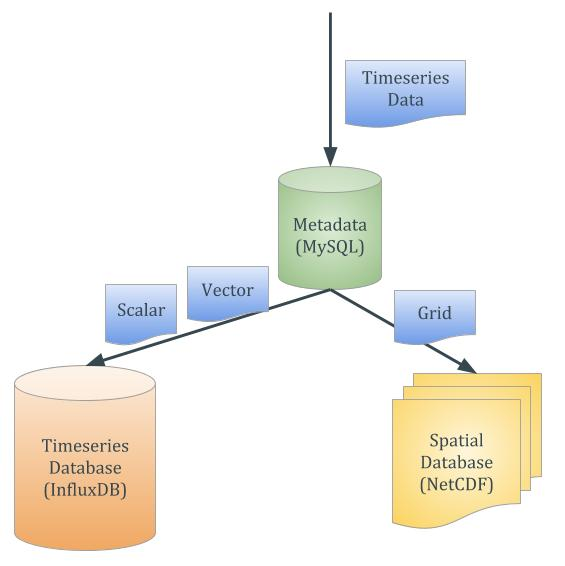
\includegraphics[width=1\textwidth]{method/microservice/hierarchical_database.jpg}
    \caption{Hierarchical Database}
    \label{fi:hierarchical_database}
\end{figure}

WDIAS is using a hierarchical database, with following the concept of Database per Service which is described in the \ref{micro_database_per_service}.
Following chapters described the usage of databases in WDIAS and reason behind the selection.

- MySQL
Relational Database Management System (RDBMS).
SQL database has fewer version of open source and it is also possible to gain better performance with commercial versions. 
Since WDIAS scope is to using open source tools, it is using MySQL as persistent database for storing timeseries metadata described above.
One instance of MySQL is using only by adapter-metadata service.
Other than that, another instance of MySQL is using for adapter-extension which will be describe in more detail \ref{data_preprocess}.
MySQL is used only for these services, those will only keep the consistency of the schema for timeseries metadata and extension metadata.
\ref{db_struct_redis} instance is using for caching the data from MySQL, since the MySQL database instances, itself not going to get much load.
Other than MySQL, there are many open source databases can be used to replace the same functionality.

- InfluxDB \cite{influxdbInfluxDBDocumentation}
Open timeseries DB with MIT license
Support SQL-Like query language
Clustering available with a commercial version
Among the other timeseries open source databases available, InfluxDB has higher number of usage and support. Database is written in Golang programming language,
and has higher performance. Other than InfluxDB, another Database is Elastic Search which is mainly using for indexing for searching.
With changing the configurations of the InfluxDB, it is possible to adapt as required. As mention in \cite{influxdbInfluxDBDocumentation}, 
InfluxDB can setup on a computer which will give the required performance. Going further, users can use commercial version of InfluxDB in order to gain more performance.

Two instance of InfluxDB is using in the WDIAS system by adapter-scalar and adapter-vector services. For the scalability, the system uses \ref{micro_database_per_service}.
But further, it split into two services, refering to the \ref{micro_z_axis_scaling} data is partitioned among few servers based on valueType key attribute of timeseries.
Which also conclude the concept of splitting into more services based on other key attributes such as timeseriesType, if further performance required.

- NetCDF \cite{unidataUnidataNetCDF}
Network Common Data Form
Self-describing, machine-independent data formats that support creation, access, and sharing of array-oriented scientific data
Support parallel file access
NetCDF is widely using in sciencetific domain due to it's capability of storing data in multi dementions easily and flexibility with storing many of the sciencetific data.
Python wrapper for NetCDF-C library using in the WDIAS system, and use by adapter-grid service.

- MongoDB
  MongoDB is a general purpose, document-based, distributed database
  Supports query operations on geo-spatial data \cite{mongodbMongoDBManual}
  Clustering and Sharding available for scalability and reliability
MongoDB geo-spatial features are using for support Geo queries in the WDIAS. Other than that, external timeseries metadata queries are served by the indexed timeseries metadata data.
If metadata not present in the adapter-query, if fetch data from the adapter-metadata, then indexed and cache in the MongoDB. Vise a versa, if new timeseries create in the adapter-metadata,
it trigger an event to adapter-query to index the new timeseries.
\ref{micro_y_axis_scaling} concept is using here by splitting into the multiple services based on the functionality and scale the system.

- Redis \cite{redisRedisDocumentation}
  Redis is an open source (BSD licensed), in-memory data structure store, used as a database, cache.
  Clustering is available for scalability
Redis uses as in-memory caching for fast access of repreative access data in adapter-metadata and adapter-extension.
Other than that, adapter-status uses Redis as key value pair store for getting the status for async handling requests such as storing Grid data.
In adapter-extension uses Redis's Publisher Subscriber capabilities in order to create a cron job in extension-scheduler when new extension create on \ref{data_preprocess}
